\documentclass[11pt]{article}
\usepackage[margin=2cm]{geometry}
\usepackage{graphicx}
\usepackage{wrapfig}
\usepackage{amsfonts, amsmath}
\usepackage{tikz}
\usetikzlibrary{positioning}
\usepackage{xcolor}
\usepackage[colorlinks = true,
            linkcolor = blue,
            urlcolor  = blue,
            citecolor = blue,
            anchorcolor = blue]{hyperref}

\usepackage{amsmath}
\usepackage{amssymb}
\usepackage{fancyhdr}
\usepackage{comment}
\usepackage{color}
\usepackage{graphicx}
\usepackage[colorlinks=true,linkcolor=blue,urlcolor=blue]{hyperref}

\newcounter{marks}
\def\maxmarks#1{\extramark{#1}\addtocounter{marks}{#1}}
\def\extramark#1{
  \begin{flushright}
  [\emph{#1 points}]
  \end{flushright}
%  \quad\mbox{\LARGE\begin{tabular}{|c|c|}
%  \hline\rule{1cm}{0cm} & #1 \\ \hline \end{tabular}}
}
\def\dumptotal{%
\begin{flushright}
\begin{tabular}{|l|} \hline
\LARGE{\textbf{\rule{0pt}{16pt}Total:~\themarks}} \\ \hline
\end{tabular}
\end{flushright}}
\def\skiplines#1{\newline \forloop{#1}{{\rule{0pt}{20pt}} \\}}

\specialcomment{answer}{\color{blue}}{\color{black}}
\def\withanswers{\def\skiplines##1{\relax}\def\skippage{\relax}}
\def\withoutanswers{\excludecomment{answer}\def\skippage{\clearpage}}

\newif\ifprint
\printtrue

\oddsidemargin0cm
\topmargin-2cm     %I recommend adding these three lines to increase the 
\textwidth16.5cm   %amount of usable space on the page (and save trees)
\textheight23.5cm  

\newcommand{\mycoursenum}{10-601}
\newcommand{\myhwnum}{4}
\newcommand{\myname}{Your Name Here}
\newcommand{\myandrew}{your-andrew-id-here@andrew.cmu.edu}
\newcommand{\myfirstta}{Qihui Li}
\newcommand{\mysecondta}{Siping Ji}

\newcommand{\question}[2] {\vspace{.25in} \hrule\vspace{0.5em} \noindent{\bf #1: #2} \vspace{0.5em} \hrule \vspace{.10in}}
\renewcommand{\part}[1] {\vspace{.10in} {\bf (#1)}}

\setlength{\parindent}{0pt}
\setlength{\parskip}{5pt plus 1pt}
 
\pagestyle{fancyplain}
\lhead{\fancyplain{}{\textbf{HW\myhwnum}}}
\ifprint
\rhead{\fancyplain{}{Andrew ID: \rule{0.2\textwidth}{.4pt}}}
\else
\rhead{\fancyplain{}{\myname\\ \myandrew}}
\fi
\chead{\fancyplain{}{\mycoursenum}}

\withoutanswers

\begin{document}

\medskip

\thispagestyle{plain}
\begin{center}
{\Large \mycoursenum: Homework \myhwnum} \\
Due: 18 October 2014 11:59pm (Autolab) \\
TAs: \myfirstta, \mysecondta \\
\medskip
\ifprint
Name: \rule{0.5\textwidth}{.4pt} \\
Andrew ID: \rule{0.45\textwidth}{.4pt} \\
\else
Name: \myname \\
Andrew ID: \myandrew \\
\fi
\end{center}

Please answer to the point, and do not spend time/space giving irrelevant details. 
%You should not require more space than is provided for each question. If you do, please think whether you can make your argument more pithy, an exercise that can often lead to more insight into the problem. 
Please state any additional assumptions you make while answering the questions. 
For Questions in this assignment, you need to submit your answers in a single PDF file on autolab, either a scanned handwritten version or a \LaTeX pdf file. 
Please make sure you write legibly for grading.
For Implementations, submit your m-files on autolab. 

You can work in groups. However, no written notes can be shared, or taken during group discussions. You may ask clarifying questions on Piazza. However, under no circumstances should you reveal any part of the answer publicly on Piazza or any other public website. The intention of this policy is to facilitate learning, not circumvent it. Any incidents of plagiarism will be handled in accordance with \href{http://www.cmu.edu/policies/documents/Academic%20Integrity.htm}{CMU's Policy on Academic Integrity}.


%%%%%%%%%%%%%%%%%%%%%%%%%%%%%%%%%%%%%%%%%%%
\question{$\star$}{Code of Conduct Declaration}

\begin{itemize}
	\item Did you receive any help whatsoever from anyone in solving this assignment? Yes / No.
	\item If you answered \emph{yes}, give full details: \rule{0.4\textwidth}{.4pt} (e.g. \emph{Jane explained to me what is asked in Question 3.4})
	\item Did you give any help whatsoever to anyone in solving this assignment? Yes / No.
	\item If you answered \emph{yes}, give full details: \rule{0.4\textwidth}{.4pt} (e.g. \emph{I pointed Joe to section 2.3 to help him with Question 2}).
\end{itemize}


\clearpage
%%%%%%%%%%%%%%%%%%%%%%%%%%%%%%%%%%%%%%%%%%%

%%\begin{document}
%%\maketitle

\section{SVM (20 points)(TA:- \mysecondta)}

In this section you will implement the polynomial and gaussian kernel, and plug in the kernel with our provided SVM implementation and test it on the dataset.
\subsection{The Dataset}

A dangerous mutant of bird flu viruses was discovered and a widespread pandemic is imminent. A vaccine was developed for improving immunity against this potent virus. However, this new vaccine is very expensive and only effective for a subset of patients. Expression of two genes X,Y are shown as predictors of the vaccine's effectiveness. You are asked to train a SVM to predict the vaccine's effectiveness on patients using gene expression measurement. Download the dataset from the course website. The .mat file contains two matrices: train and test. There are 160 training examples and 40 testing examples. The dataset used in this section has two dimensional features (it's better for you to first visualize the data and see which SVM kernel makes sense). The task is to use SVM with different kernels to perform binary classification. 

\subsection{Training SVM}

Given a set of training points $x_1, x_2, ..., x_m$ and a set of labels $y_1, ..., y_m$ we want to maximize the margin between decision boundary and support vectors. By incorporating slack variable, the model is more flexible for handling non-separable cases. The constrained optimization problem can be formalized as following:

\begin{align}
min~~~~~~~C\sum_{n=1}^N{\xi_n} + \frac{1}{2}||\textbf{w}||^2~~~~~~~~~~~~~~~~~~~~~~~~~~\\
s.t. ~~~~~~~~~y(x_n)t_n \geq 1 - \xi_n, ~~~~~~~~~~n=1,...,N\\
     \xi_n \geq 0,~~~~~~~~~~~~~~~~n=1,...,N
\end{align}

where C $\geq$ 0 is a parameter that controls the trade-off between the slack variable
penalty and the margin.

\subsection{Kernel Trick}
Kernel functions can be used in SVM to classify linearly inseparable data in implicit hight dimensional feature space without making explicit feature mapping. Here are several kernel functions that are commonly used.
\begin{align}
Polynomial:~~~~~~~~~~ (x_i \cdot x_j + 1)^d~~~~~~~\\
Gaussian:~~~~~~~~~exp(-\gamma||x_i - x_j||^2)
\end{align}


\paragraph{(20 points) Implement the kernel functions.} Here we already provide you with a svm implementation where you can easily plug in the kernel function. Please implement the polynomial in \textbf{polynomial\_kernel.m} and gaussian kernel in \textbf{gaussian\_kernel.m }and have them tested on the dataset we provide to you. \textbf{Note:} Under folder svm, function \textbf{svm\_train.m} and \textbf{svm\_classify.m} is provided for training and testing phase of svm. A \textbf{svm\_runner.m} is also provided to you as an example for accessing these interfaces. If octave complains about the qp solver please use the commented statement in svm\_train instead. 

\section{Compare Classifiers (80 points)(TA:- \myfirstta)}

%\begin{wrapfigure}{r}{0.5\columnwidth}
%\label{bananaset}
%\begin{center}
%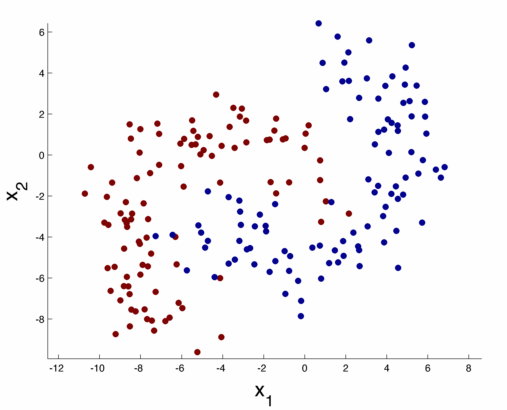
\includegraphics[width=0.5\columnwidth]{./figures/banana_dataset.png}
%\end{center}
%\caption{Banana dataset. Created from two intertwined banana shaped distributions. Red is class 1 %and blue is class 0. It is not possible to classify this dataset well using a 2D linear classifier.}
%\end{wrapfigure}
 In this part we'll implement several measures for evaluating the performance of classifier. Now that we have learned and implemented several supervised machine learning algorithms, we may wonder how well a certain classifier performs and how they perform against each other regarding a certain problem. We already know we can compare their classification accuracy on a held out test set. But is it a robust measure? Would the result be different if our selection of held out test set is different? 

You have three tasks in this section.

\begin{enumerate}
\item Implement a function for calculating \textit{Confidence Interval} .
\item Implement functions performing test on \textit{Held-out Set} and test on \textit{Cross Validation} and obtain confidence interval under these 2 tests with the SVM algorithm you've implemented on the vaccine dataset in section 1.
\item Use \textit{t-test} for comparing classifiers and compare Logistic Regression with Neural Network performances on the MNIST dataset from home work 3.

\end{enumerate}

\subsection{Confidence Interval}

Beside the accuracy, now you also have to output a confidence interval for the accuracy. Here is a detailed tutorial of  $\href{http://nbviewer.ipython.org/github/demotu/BMC/blob/master/notebooks/ConfidencePredictionIntervals.ipynb}{Confidence Interval}$. You should compute confidence interval based on the formula given below:
$$[Accuracy_s(h)- Z_n \sqrt{Accuracy_s(h)(1-Accuracy_s(h)/n} , Accuracy_s(h)+Z_n\sqrt{Accuracy_s(h)(1-Accuracy_s(h)/n}$$
where $Accuracy_s(h)$ is the accuracy on sample set from hypothesis h, in this case the sample set is the test set. $Z_N$ is the appropriate number of standard deviation corresponding to the interval level N in Normal distribution which can be looked up in a table, and n is the size of testing set. A $Z_N$ (z-score) look up table is provided $\href{https://people.richland.edu/james/lecture/m170/ch08-int.html}{here}$.

\paragraph {(10 points)Implement the \texttt{ConstructInterval} functions.} For this task you need to implement function [Accuracy, lowerInterval, upperInterval] = ConstructInterval(Ypredict,Ytest,confLevel). You only need to compute confidence interval of confidence level 99\% and 95\%.

\subsection{Test on Held-out set }

One strong assumption for constructing confidence intervals is that the classifier should be independent from the testing set. (Otherwise it will almost always optimistically biased.)  \newline
One way to enforce independence is to draw a partition from training data as testing set and "hold out" this partition during training, so that it is not seen by the classifier learner. However, holding out too much data will weaken the accuracy of the classifier (there is less data in training), while drawing too little data will weaken the accuracy of the test (and lead to a wider confidence interval). 

\paragraph {(0 points)Implement the \texttt{PartitionHeldOut} functions.} For this task you need to implement function   \texttt{testInstanceLabel = PartitionHeldOut(size, k)} where size is the number of instances in the set and k is the number of partitions you wish to do.  Your output testInstanceLabel is a binary vector where its elements is either 0 or 1, indicating which instances are used as testing set. The size of it is the number of instances in the set.
In PartitionHeldOut function, you partition the set into k subsets of equal size randomly. You select one of them as your testing set by labelling the corresponding elements of the subset in testInstanceLabel as 1 and the rest as training set by labelling the rest elements in testInstanceLabel as 0.

\paragraph {(20 points)Implement the  \texttt{TrainHeldOut functions}.} For this task you need to implement function   \texttt{Ypredict = TrainHeldOut(Xtrain, Ytrain, testInstanceLabel)}. In TrainHeldOut function, testInstanceLabel is a binary vector to indicate the training set and testing set. You should use Naive Bayses classifier you implemented in home work 2 for this. Your output Ypredict will only contain test part of instances. \newline

\paragraph{(10 points) Question} Combine the train and test sets of the vaccine dataset in section 1as new training dataset. The new training dataset should have 200 instances in total. Using no kernel (or $\phi $$(x_n) = x_n$)), train a SVM using C = 0.5. Calculate 95\% and 99\% confidence interval on number of partition 2 and 10 on new training dataset. Describe in one sentence what you observe in the result.

\subsection{Test by Cross-Validation}
In order to get more testing data, one way is to do cross-validation. For a 10-fold cross- validation, you train the model 10 times, each time using a different 1/10 data as the testing
set. In the end, every data point has one prediction (since it was used exactly once as a test case), and we can get the prediction accuracy on the whole training set to construct a confidence interval.
Note that for each model, though the classifier is independent from the testing data, those 10 models are actually dependent (due to overlap with the training set). However, in practice, this usually a good approximation.
%For this section, try 2-fold and 10-fold cross-validation and report their 95\% and 99\% confi- dence %intervals respectively.

\paragraph {(0 points)Implement the  \texttt{PartitionCrossSet} functions.} For this task you need to implement function   \texttt{YcrossSetLabel = PartitionCrossSet(size,k)}.
In PartitionCrossSet, you randomly assign instances to one of k sets, and every set should have (as close as possible to) the same number of instances. crossSetLabel is a vector contains number from 1 to k, which indicates the set the instances belong to.

\paragraph {(20 points)Implement the  \texttt{TrainCrossSet} functions.} For this task you need to implement function   \texttt{Ypredict = TrainCrossSet(Xtrain, Ytrain, crossSetLabel)}.You should use Naive Bayses classifier you implemented in home work 2 for this. You can call TrainHeldOut from your TrainCrossSet. In TrainCrossSet, crossSetLabel indicates how you segment the data to k sets, you should train model k times and every time one partition will be the testing set. Therefore, the size of Ypredict should be the same as Ytrain.

\paragraph{(20 points) Question} Combine the train and test sets of the vaccine dataset in section 1 as new training dataset. The new training dataset should have 200 instances in total.Using no kernel (or $\phi $$(x_n) = x_n$)), train a SVM using different values of C = 0, 0.1, 0.3, 0.5, 1, 2, 5, 8, 10. Use 4-fold cross validation and report the train and test errors. Produce a plot of 2 curves: training and testing error. The x-axis shows different values of C and the y-axis shows the error rate. \newline
Which value of C yields the best training and testing error rate? Which value of C should you use?
\subsection{P Values and t-tests}

P Values and t-tests are statistical measures for determining the significance of an an event. A detailed tutorial can be found $\href{https://www.csulb.edu/~msaintg/ppa696/696stsig.htm#Using\%20t}{here}$.\newline
To systematically evaluate two classifiers without possible random bias in comparison, we need to look at whether the performance of one classifier is significantly better than the other by statistical measures. \newline
The method is described below. \newline \newline
Divide the testing set into k disjoint subsets. For each subset $T_i$, we compute the difference of error rates from two classifiers.
$$ Y_i = error_{t_i}(h1)  - error_{t_i}(h2)$$
Each $Y_i$ is a random variable, so the average $\bar{Y} = \frac{1}{k} \sum_{i=1}^{k}Y_i$ is also a random variable. When k $\geq$ 30, the random variable Y approximates a normal distribution. But if k $<$ 30, it can be approximated as t-distribution with k-1 degrees of freedom. 

In the next step, we set a null-hypothesis that $E[\bar{Y}] = 0$. If we can reject this null-hypothesis by two-tail test, it means one classifier is better than the other (either h1 or h2 is better). Or, by one-tail test, we can test if the a specific h is better than the other.

For example, when a given k, and null hypothesis $E[\bar{Y}] = 0$, t-value will be
$$ \frac{\bar{y}\sqrt{k}}{S_k}$$
$$ S_k^2 = \frac{1}{k-1}\sum_{i=1}^{k}(y_i-\bar{y})^2$$
Then we can see whether we can reject the null hypothesis under different significance levels. \newline


%\paragraph {(10 points)Implement the  \texttt{CompareClassifier}.} For this task you need to i%mplement function   \texttt{[accuracy1, accuracy2, pvalue] = CompareClassifier(Ypredict1,Ypredict2, %Ytest, crossSetLabel,isTwoTail)}.For CompareClassifier, you should have same length for Ypredict1 %and Ypredict2. crossSetLabel indicates the set each instances belong to. Ytest is the true label for %Ypredict1 and Ypredict2. When IsTwoTail = 1, you should perform two-tailed test, otherwise you %should perform one-tailed test. For accuracy, you should show the overall accuracy for both classifiers.

%\paragraph{(5 points) Question} A script runNNClassification.m is provided to you for running Neural %Network on the new vaccine dataset. Replace the old script with the new one and describe what %you've found comparing the result you obtained from Neural Network with the result you obtained by %running SVM in the last question. \textbf{Note: You should implement this test yourself, and not use %matlab function ttest directly. For mapping t-value to p-value, you can use the matlab function %\textit{tcdf}.}


\paragraph{(10 points) Question} Use the best set of parameters you've found for Logistic Regression and NN on the MNIST data set from home work 3. Compare Logistic Regression and NN, report their accuracy and p-value under one-tailed test and two-tailed test with k=10. Reason about what you found in two sentence.\newline \textbf{Note: You should use the matlab function \textit{ttest} directly. }
 \newline 
 \section{Deliverables}
 Submit your codes in four parts via AutoLab. You can use the your codes from previous assignments as classifiers. You are NOT allowed to use any off-the-shelf optimizer. You should upload your codes (including all your function files) along with a report, which should solve the questions above.\newline
You should tar gzip the following items into hw4part1.tgz and submit to the Homework 4 - Construct Interval under Autolab:
\begin{itemize}
\item ConstructInterval.m
\item and all other auxiliary functions you have written 
\end{itemize}
You should tar gzip the following items into hw4part2.tgz and submit to the Homework 4 - Cross-Set + Held-Out under Autolab:
\begin{itemize}
\item TrainHeldOut.m
\item TrainCrossSet.m
\item and all other auxiliary functions you have written 
\end{itemize}
You should tar gzip the following items into hw4part3.tgz and submit to the Homework 4 - SVM under Autolab:
\begin{itemize}
\item polynomial\_kernel.m
\item gaussian\_kernel.m
\item and all other auxiliary functions you have written 
\item report.pdf
\end{itemize}
Please submit a file called \texttt{hw4part3.tgz}. Please place all your code in a folder \texttt{hw4part3} and then tar the folder using the following instructions : \newline
Tar gzip the files directly using \texttt{tar -cvf hw4part3.tgz *.m report.pdf}. Do NOT put the above files in a folder and then tar gzip the folder. You do not need to upload the saved predicted labels (i.e. the .mat files). Please make sure your code is working fine under Octave before you submit.\newline \textbf{Note:  You should not include \textit{svm\_train.m} \textit{svm\_classify.m} \textit{svm\_runner.m} \textit{Partition\_CrossSet.m Partition\_HeldOut.m nb\_train.m or nb\_test.m} in hw4.tgz though you do need to call these functions in the files you submit. }

%\textbf{Note: You should not include Partition_CrossSet.m Partition_HeldOut.m nb_train.m or nb_test.m  in hw4.tgz though you do need to call these functions in the files you submit. }

\end{document}
